\newpage
\section{Envelopes for Curves}

In this activity, we'll investigate how we actually make curves via
envelopes of tangents.


\begin{prob}
Consider the following curve:
\[
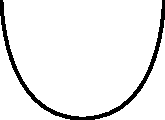
\includegraphics{../graphics/envU.pdf}
\]
Use 7-line envelope of tangents to draw this curve in the provided
grid:
\[

\includegraphics{../graphics/complexPlane.pdf}
\]
\end{prob}


\break


\begin{prob}
Consider the following curve:
\[
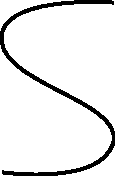
\includegraphics{../graphics/envS.pdf}
\]
Use 7-line envelope of tangents to draw this curve in the provided
grid:
\[

\includegraphics{../graphics/complexPlane.pdf}
\]
\end{prob}

\break

\begin{prob}
Consider the following curve:
\[
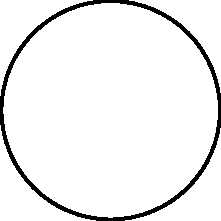
\includegraphics{../graphics/envO.pdf}
\]
Use 7-line envelope of tangents to draw this curve in the provided
grid:
\[

\includegraphics{../graphics/complexPlane.pdf}
\]
Check your solution with a compass---what do you find?
\end{prob}

\break

\begin{prob}
Consider the following curve:
\[
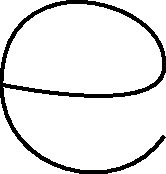
\includegraphics{../graphics/envE.pdf}
\]
Use 7-line envelope of tangents to draw this curve in the provided
grid:
\[

\includegraphics{../graphics/complexPlane.pdf}
\]
\end{prob}
